\section{Development Process}

The following section aims to analyze and offer insight into the development process of the project. Key elements such as the mechanical design of the gripper, component selection, the kinematics of the UR robot, and the interfacing of the different subsystems will be dissected. 

\subsection{Mechanical Design} 
Anders og Magnus.

The final design of the gripper utilizes gears to move the fingers in a claw-like fashion. This choice is based needing smooth motion whilst working with a rough and imprecise material such as PLA. The gears also allow for the use of just one motor. The first motor used was a high geared DC motor, that was supposed to use a current sensor to determine when to open and close. However, this proved difficult (see section XXX), so a different motor was tested. The final motor choice for this application is a servomotor, due to its ease of use and its precision regarding the rotor's angular displacement. This works because the motor runs on a closed-loop control system receiving Pulse-Width Modulation (PWM) signals. The internal potentiometer registers the actual mechanical position of the shaft, and creates a feedback signal. Then an error is calculated,; the discrepancy between the reference signal and feedback signal. Subsequently, the error is minimized with an integrated PID controller.\cite{Servo}  
\\ 

The overall design was made slim, taking up only the utmost necessary amount of space. This design choice had multiple benefits: It takes less time to 3D print and there is less risk of the gripper accidentally colliding with the construction, while still allowing enough room for the indispensable components such as the camera needed for computer vision. A second key feature of the gripper design is that there is a joint between the finger and the fingertip, resulting in increased dexterity and versatility when it comes to picking up objects of different shapes and sizes. A small but important detail is the rail that runs along the base of the gripper. This rail ensures alignment between the two gears, and that they do not loosen and fall off. 
\\
\begin{figure}[H]
    \centering
    \begin{minipage}{0.48\linewidth}
        \centering
        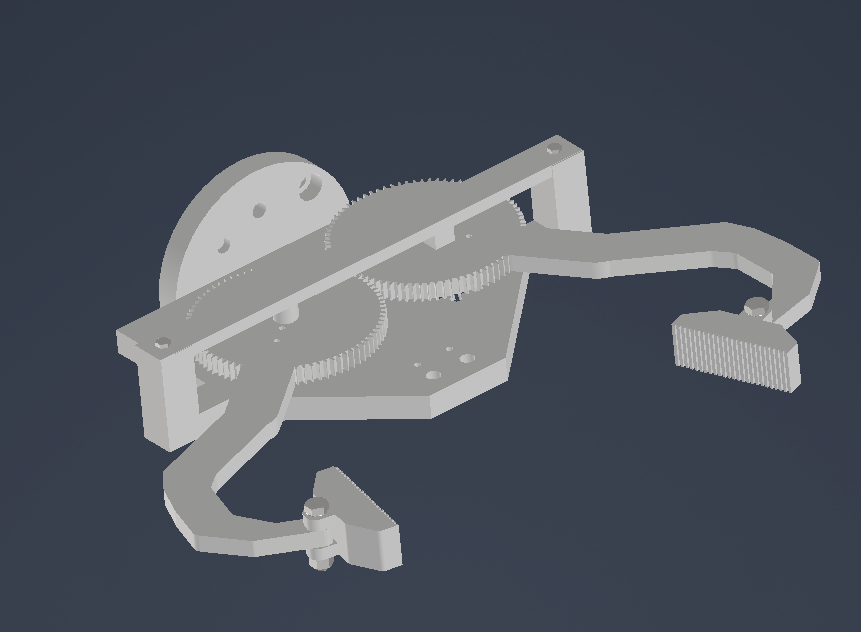
\includegraphics[width=\linewidth]{Report/pictures/Servo1.png}
        \caption{Final servo motor gripper}
        \label{fig:servo_final}
    \end{minipage}
    \hfill
    \begin{minipage}{0.48\linewidth}
        \centering
        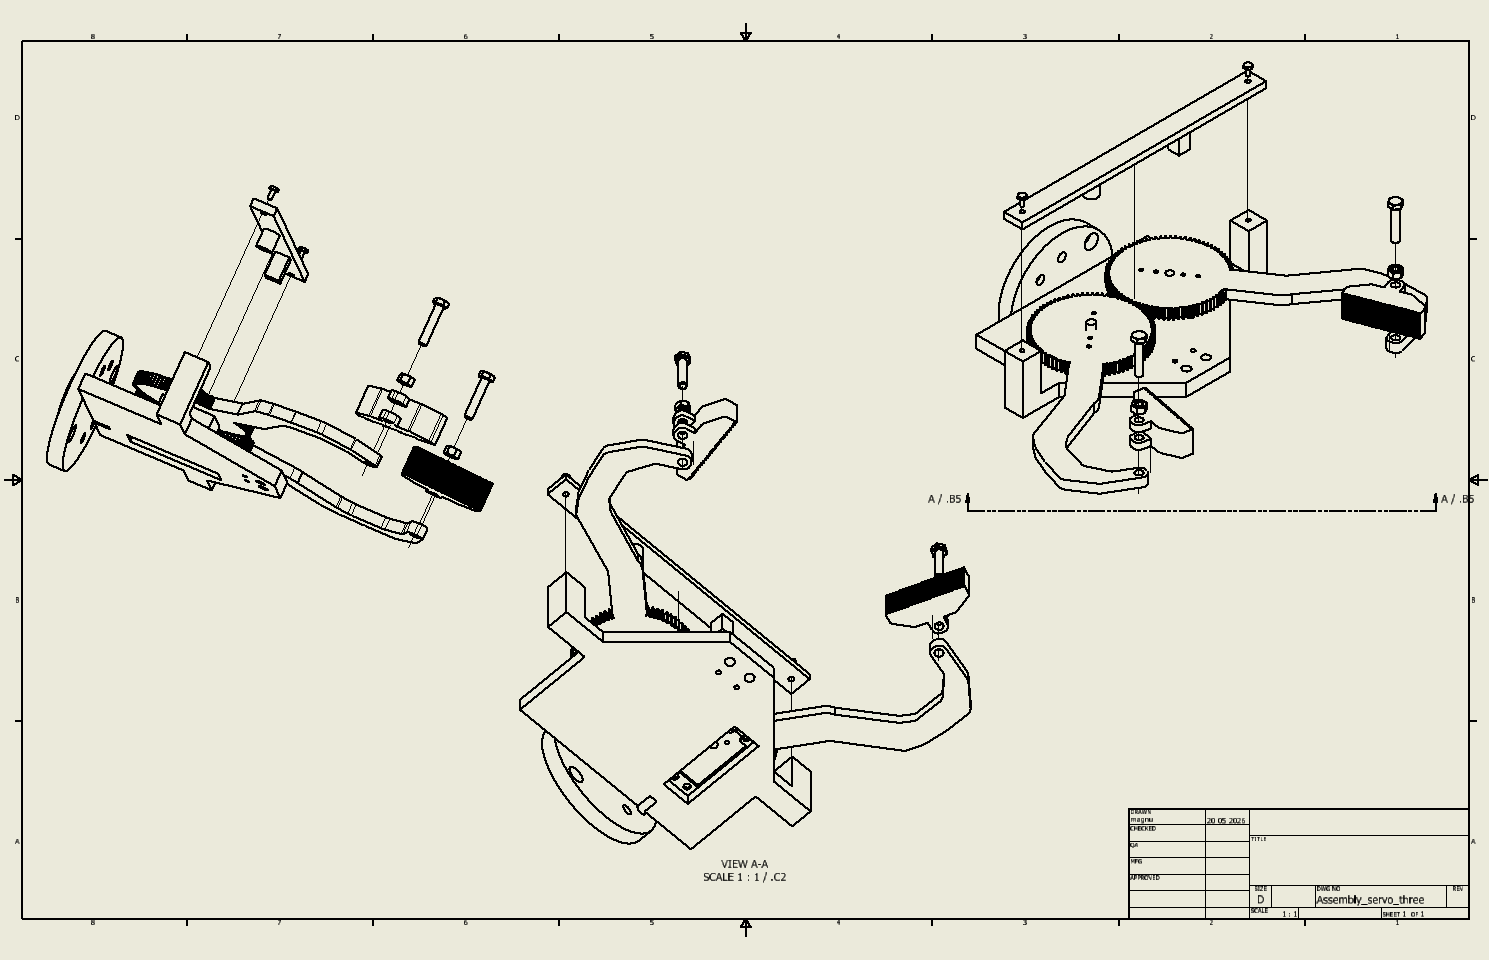
\includegraphics[width=\linewidth]{Report/pictures/Servo.png}
        \caption{Servo from different angles}
        \label{fig:servo_three}
    \end{minipage}
\end{figure}

Conversely, the first gripper design was a parallel gripper with a bulky base. The idea was that it needed to be able to store all the necessary electrical components. The main issue with the design was the mechanism, where the mechanical binding caused by plastic-on-plastic friction resulted in the fingers getting stuck when pulled through the track clearance gaps. To alleviate this friction issue, the clearance gaps were made bigger to better accommodate the fingers. Unfortunately, this introduced a new problem; the fingers would twist out of alignment, and this angular misalignment caused them to get wedged and jam during operation. This resulted in another being the DC motor would rotate endlessly inside of the gripper due to the jamming caused by the Plastic.This forms the basis of the gripper choice and why the claw-like mechanism reigned superior in this case. \\

ANDERS SKAL DER VÆRE BILLED HER?????

To test the efficacy of the gripper, an experiment was conducted to see which shapes the gripper was able to pick up. The parameters of the experiment were as follows: The gripper was moved linearly up and down to pick up each object, and held on to the object for 3 seconds, before being put back down. Each shape was tested 10 times and the results can be seen in Table 2.

\subsubsection{The Servo tests }


\begin{table}[H]
    \centering
    \caption{Gripper pick-up shape test}
    \label{tab:gripper_test_matrix}
    \begin{tabular}{| p{3.5cm} | p{2.2cm} | p{2.2cm} | p{5.5cm} | c |} 
        \hline
        \textbf{Block Type} & \textbf{Dimensions (mm)} & \textbf{Mass (g)} & \textbf{Test Scenario / Surface Texture} & \textbf{Result} \\ \hline
        % Row 1: Smooth PLA
        Standard Cube & $50 \times 50 \times 50$ & $40\text{g}$ & Smooth surface. Low friction. & 10/10 \\ \hline
        % Row 2: 
        Standard Cube (angled) & $50 \times 50 \times 50$ & $40\text{g}$ & Cube is put an a 45 degree angle. & 9/10 \\ \hline
        % Row 3:
        Large Rectangular & $100 \times 50 \times 50$ & $42\text{g}$ & Smooth surface. Low friction. & 10/10 \\ \hline
        % Row 4: 
        Triangle & $b=50, h=50, l=50\text{ mm}$ & $17\text{g}$ & Smooth surface. Low friction. Picked up at the hypotenuse. & 0/10 \\ \hline
        % Row 5: 
        Triangle (with duct tape on the hypotenuse) & $b=50, h=50, l=50\text{ mm}$ & $17\text{g}$ & Textured surface due to duct tape, offering more friction. Picked up at the hypotenuse. & 10/10 \\ \hline
        % Row 6: 
        Wooden hollow box (with duct tape) & $110 \times 30 \times 60$ & $118\text{g}$ & Smooth wooden surface. Low friction.. & 8/10 \\ \hline
        % Row 7: 
        Metal Puck (with duct tape) & $\varnothing 50 \times 20\text{ mm}$ & $744\text{g}$ & Smooth metal surface. Low friction & 0/10 \\ \hline
      
       
    \end{tabular}
\end{table}


The test indicates that the gripper is very effective at picking up various shaped objects, even at odd angles. However, the gripper was only able to pick up the triangle when tape was applied to both the gripper fingers and the triangle's hypotenuse, due to the smooth surface. Which illustrates the importance of grip for this application. The goal was to make the final iteration with a softer, rubbery material like TPU on the finger tips, so that the gripper could shape itself after the object, but due to time constraints, this was not tested. \\

As seen in Table 2, a very heavy metal object was attempted to be picked up and failed. Nevertheless, this led to a different experiment to see the gripper's load bearing capabilities.



\begin{table}[H]
    \centering
    \caption{Gripper Maximum Weight and Load Capacity Testing}
    \label{tab:load_capacity_test}
    \begin{tabular}{| c | c | c | p{7.5cm} |} 
        \hline
        \textbf{Test Iteration} & \textbf{Added Mass (g)} & \textbf{Total Mass (g)} & \textbf{Observations / Failure Mode Analysis} \\ \hline
        % Test 1
        1 & $0\text{g}$ & $118\text{g}$ & Base weight of the hollow box shell. Lift executed 8/10 times. \\ \hline
        % Test 2
        2 & $74\text{g}$ & $192\text{g}$ & Nominal load. Smooth acceleration and stable retention. Lift executed 10/10 times. \\ \hline
        % Test 3
        3 & $80\text{g}$ & $272\text{g}$ & Nominal load. Good and stable grip. Lift executed 10/10 times. \\ \hline
        % Test 4
        4 & $66\text{g}$ & $338\text{g}$ & Minor slip detected during initial testing, but gripper recovered. Lift executed 10/10 times.  \\ \hline
        % Failed Test (Highlighted in light red)
        \rowcolor{red!15} 5 & $12\text{g}$ & $350\text{g}$ & \textbf{FAILURE:} The hollow box slipped entirely out of the fingers due to insufficient clamping torque and grip. 0/10. \\ \hline
    \end{tabular}
\end{table}

The load bearing experiment demonstrated that the maximum weight the gripper can consistently lift is $ \sim 338\text{ g}$. That proved plenty for this application, as the blocks used only weighs about 40 g. However, if heavier blocks were needed for the project, one way to increase clamping torque would be to supply the motor with more current. When testing, both 0,7 amps and 1 amp was used to see what difference it makes, and the load capacity increased nearly twofold going from 0,7 amps to 1 amp. The aforementioned DC motor would have significantly more torque due to its high gearing, but due to the issues the motor caused, as well as the time constraints, it was not possible to test its full loading capacity for comparison. Furthermore, shorter fingers for the gripper would also theoretically provide more clamping force as the force applied is torque (T) divided by distance (d).
$$F = \frac{T}{d}$$

The downside is less versatility in what objects it can pick up, as shorter fingers would struggle to pick up larger objects. It is hypothesized that the first designed parallel gripper would have a higher loading capacity due to the 90 degree contact angle, had it worked. This mechanism ensures all the clamping force goes into the object and maximizes grip. For the mechanism to work, miniature metal guiding rails could be implemented to eliminate the plastic-on-plastic friction, resulting in a smoother actuation path while concurrently preventing jamming under heavier loads.




\subsubsection{Partial Conclusion}
The general thesis was to create more than one design, to compare the different designs to come to an final outcome being the best design. 

Our final designs involves two different ones a claw design and the other being an parallel gripper which in theory should be able to lift a heavier load than the other one, however our design had to much friction and problems with the DC motor usage that the only solution to solve this problem was to make it out of another material rather than plastic. This will be more talked about in improvements.\\

Due to this reason reason including ease of usage of the other the claw design, was the best outcome for our application being picking of light weight object. 








TESTS (MIKKEL, Anders og Magnus).







\subsection{Electrical Components and Circuitry} 
jeppe, gustav og nicolai.


\subsubsection{Spectral Sensor}
Nicolai
For color detection, a spectrometer (AS7341) from Adafruit(1) was used. The AS7341, is a 10-channel spectral sensor, capable of resolving light intensity across 10 distinct wavelength bands. It is able to measure in the range from approximately 350nm to 1000nm(2). The 10-channels consist of 8 visible light channels, one NIR (Near infrared) and a clear channel with no filter(3). 
\begin{figure}[H]
    \centering
    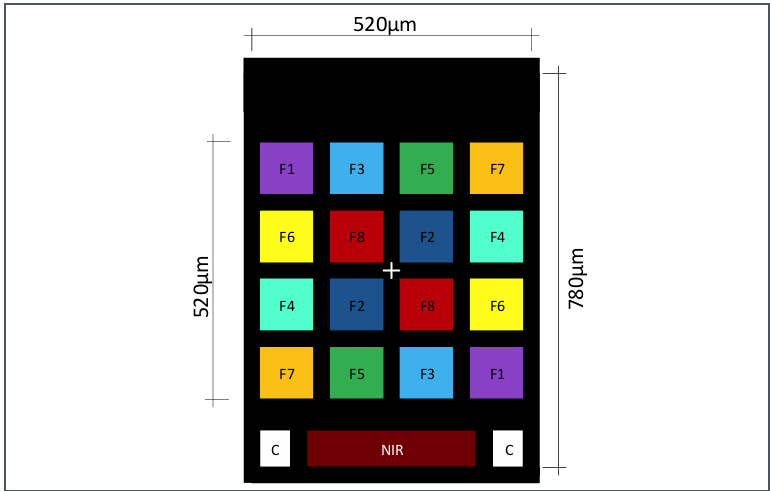
\includegraphics[width=0.5\linewidth]{Skærmbillede 2026-05-20 110202.png}
    \caption{Enter Caption}
    \label{fig:placeholder}
\end{figure}

Since the AS7341 has 10 channels but only 6 internal ADC’s, it utilizes a SMUX (spectral multiplexer). The SMUX, is an internal switchboard that decides which channels are connected to the ADC’s during each measurement cycle (5).
But one of the most important functionalities of the AS7341. Is the integration time, the integration time decides how long the photodiodes collect photons. And can therefore be adjusted depending on the intensity of the light hitting the sensor. The integration time defined by this formula (6):

$t_{int} = (ATIME + 1) * (ASTEP + 1) * 2.78 \mu_s
(t_{int} = time to integration)$

Doing the first phases of designing and making the sensor work, it was noted that there were extreme readings on the red channels F7 and F8. While the green (F4 and F5) and blue (F2 and F3) channels. The readings were on around 60-70\% of the light detected, while the green and blue were around 15-20\% each. 
It was then later decided that by actively forcing the red down by around 35-40\%, then blue and green began to be detected sometimes but not often. 
In the final design, it was made with a casing around the sensor to try and shield it from external light sources, since red light is a big part of the visible spectrum. 

To test how effective the spectral sensor AS7341 is, it was mounted with the casing on the gripper. It was then tested to see how effective the sensor was at detecting different colors over two different distances 10 cm and 20 cm over the table. These different distances were chosen since they were the most likely distances to the table when running everything together.

\subsubsection{Spectral Sensor test}
Nicolai

AS7341 distance and color detection test:


\begin{table}[H]
\centering
\caption{10 cm to table and 6 cm to block ($t_{int} = 41.7$ ms)}

\resizebox{\textwidth}{!}{%
\begin{tabular}{|c|c|c|c|c|c|c|c|c|}
\hline
\textbf{Color of blocks} & \textbf{Measurements} & \textbf{Avg. red value} & \textbf{Avg. green value} & \textbf{Avg. blue value} & \textbf{Avg. red \%} & \textbf{Avg. green \%} & \textbf{Avg. blue \%} \\ & \textbf{Avg. green value} & \textbf{Avg. blue value} & \textbf{Avg. red \%} & 
\textbf{Avg. green \%} & \textbf{Avg. blue \%} \\
\hline
Red  & 50 & 4210 & 3200 & 3990 & 36.4\% & 27.8\% & 34.8\% \\
Blue & 50 & 4185 & 3202 & 3917 & 36.2\% & 28.0\% & 34.9\% \\
\hline
\end{tabular}%
}
\end{table}

\begin{table}[H]
\centering
\caption{20 cm to table and 16 cm to block ($t_{int} = 41.7$ ms)}

\resizebox{\textwidth}{!}{%
\begin{tabular}{|c|c|c|c|c|c|c|c|c|}
\hline
\textbf{Color of blocks} & \textbf{Measurements} & \textbf{Avg. red value} & \textbf{Avg. green value} & \textbf{Avg. blue value} & \textbf{Avg. red \%} & 
\textbf{Avg. green \%} & \textbf{Avg. blue \%} \\
\hline
Red  & 50 & 4093 & 3187 & 4044 & 35.5\% & 27.9\% & 35.6\% \\
Blue & 50 & 4054 & 3197 & 4018 & 35.4\% & 28.2\% & 35.4\% \\
\hline
\end{tabular}%
}
\end{table}

\subsubsection{Current Sensor}
jeppe.

\subsection{}

\subsection{Computer Vision}
Magnus og Anders.

Computer Vision was an integral part of the overall system. A camera was mounted on the gripper base which in turn captures an image of the whole workspace to locate the objects and calculate the exact coordinates needed for the kinematic computations. At first the idea was to identity the colors of each object, create bounding boxes of said objects, so that the application adhered to the requirements stated in section XXX. This resulted in a lot complexities as the the lighting conditions and distance to the objects varied, which led to inaccuracy in the system. Hence the idea was scrapped and it was decided to use ArUco (Augmented Reality University of Cordoba) markers instead. They are simple a binary square with a black background, that a program can be calibrated to find using OpenCV.\cite{ArUco} OpenCV was used as the computer vision framework due to being highly optimized for C++ application as well as its ability to compute matrices and geometry algorithms in real time. 

The benefits of using fiducial ArUco markers are that they offer very reliable and accurate object localization, even with variable lighting conditions or partial occlusion. Furthermore, post calibration, the detection algorithm can compute the 3D orientation and position from the camera's point of view. This is called pose estimation and provides the pitch, roll, and yaw (XYZ axes) from the center of the marker relative to the gripper. The marker was then placed on the corner of a tray, on which, the different shaped blocks was sitting on (see section Grid and Blocks). 

\subsubsection{Calibration}

As mentioned, in order for the camera to detect the marker accurately, it needs to be calibrated first. The calibration is done to correct for the lens distortion and to validate the intrinsic camera parameters. A checkered paper is printed with predefined grid dimensions and is placed on a flat surface, whereafter pictures of said grid are taken at various angles, distances, and rotations and computed with OpenCV's algorithm. To evaluate the accuracy of the calibration, the RMS (Root-Mean-Square) error was used as a standard metric. Any value $>1.0$ is considered unacceptable, and thus it took several calibration attempts to obtain an RMS value of $\sim 0.8$, which is considered acceptable. By analyzing the displacement of the grid vertices the algorithm can calculate the Intrinsic Matrix and the Distortion Coefficients which is then exported to a .yml file, which allows the main system to use that data to rectify the displacements and for better accuracy when it comes to the pose estimation.  






\subsection{Robotmovement}
To bind the gripper, computer vision and grid system together, a general robotic movement system is needed. Forward kinematics is used to express all coordinate frames relative to each other — from the gripper flange to the tray and grid. An inverse kinematics based path planning system is then used to determine which joint configurations the robot should take to reach a given target position in a linear motion.
\subsubsection{TCP target transformation chain}
\begin{figure}[H]
    \centering
    
\includegraphics[width=1\textwidth]{transformation_chain.pdf}
    \caption{The figure shows the TCP target transformation chain of the robot. The top of each element shows the transformation matrix notation, and the bottom shows the corresponding values — either constant if fixed, or a variable if the value changes at runtime.}
    \label{fig:mit_billede}
\end{figure}

In figure \ref{fig:mit_billede} the TCP target transformation chain can be seen, describing the rotations and translations from the robot's base to the target TCP position. The first transformation accounts for the rotation between the robot's base frame and the world frame, which in our setup is a 156° rotation based on the robot's physical placement. The second transformation describes the position and orientation of the grid relative to the base frame — this is the grid from which the robot picks or places objects. The third transformation is expressed from the grid's perspective and defines the concrete goal position, i.e. where on the grid an object should be placed or picked. The fourth transformation accounts for the tool flange, which has a constant rotation and translation derived from its CAD design, with an additional rotation around the z-axis used to rotate the gripper while keeping the block's orientation relative to the tool flange. The tool flange transformation is applied as an inverse, resulting in a reverse translation, since the robot's forward kinematics is described from the base to the tool flange.

\subsubsection{pathfinding}
The output shown in figure \ref{fig:mit_billede} is used as input to a function called \texttt{findPath(startPose, goalBase, startAngle)}, which takes the robot's current TCP pose, joint configuration, and a target coordinate, and performs three steps. First, it discretizes the path between the start and goal position into points spaced 3 cm apart. Second, it computes all inverse kinematics solutions for each point, filters out solutions that violate joint constraints, and marks points with no valid solution as singularities. Third, it selects the joint solution for each point that takes the shortest rotational path between each point.
\begin{figure}[H]
    \centering
    \begin{subfigure}[t]{0.49\textwidth}
        \centering
        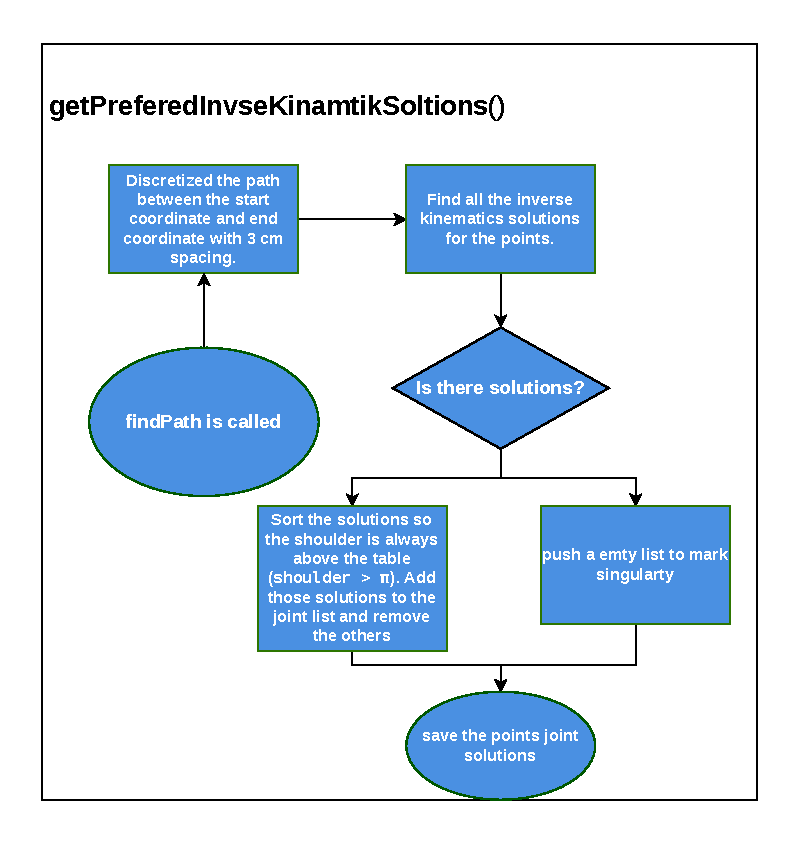
\includegraphics[width=\linewidth]{pathfin1.pdf}
        \caption{Flow diagram showing how the system finds and sorts joint solutions and filters singularities}
        \label{fig:pathfind1}
    \end{subfigure}
    \hfill
    \begin{subfigure}[t]{0.49\textwidth}
        \centering
        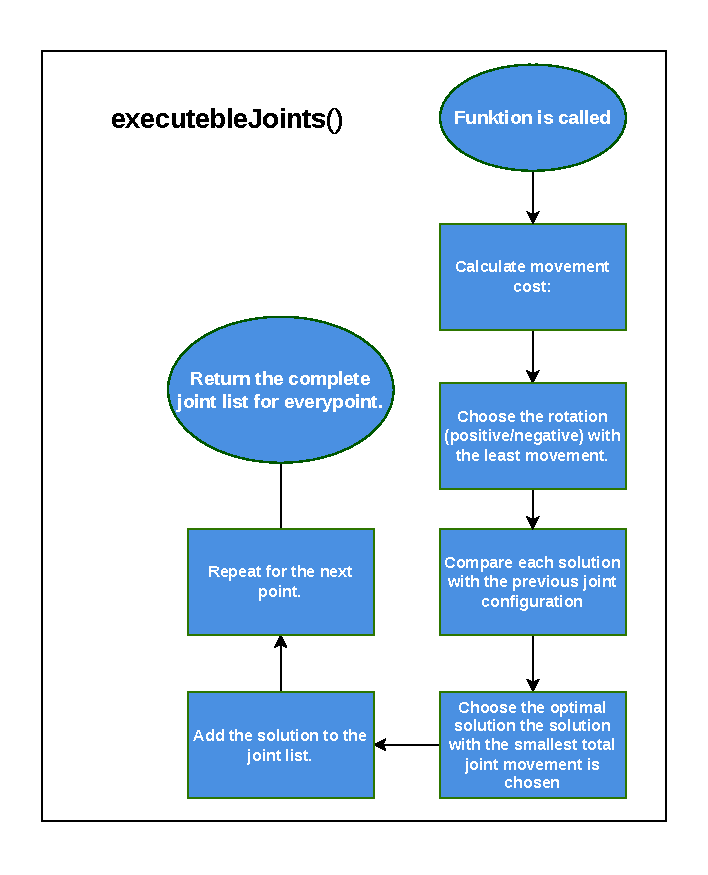
\includegraphics[width=\linewidth]{pathfind2.pdf}
        \caption{Flow diagram showing how the system find the shortes joint confiration between points}
        \label{fig:pathfind2}
    \end{subfigure}
    \caption{Path finding flow diagrams}
    \label{fig:pathfind}
\end{figure}
As the linear discretization of the path is a straightforward function, it will not be elaborated further. An overview of the solution-sorting function can be seen in Figure \ref{fig:pathfind1}. The function works as follows: an external library called \texttt{urkinematics} provides the forward kinematics and an analytical inverse kinematics solver for the robot. Since there are at most 8 possible solutions, 2 elbow, 2 wrist, and 2 shoulder configurations. That's makes it possible to filter solutions and control how the robot reaches a position by setting joint limits. In this implementation the shoulder is constrained to 0-180 degrees. This removes solutions that would cause the robot to collide with the table.
This also allows the system to pass through singularities by shifting to joint space between path points, which mostly occur when the robot loses a degree of freedom. After filtering, \texttt{executeableJoints} takes the previous joint configuration as input and finds the best solution at each point such that the total joint displacement is minimized, as can be seen onFigure \ref{fig:pathfind2} .
\begin{figure}[h]
    \centering
    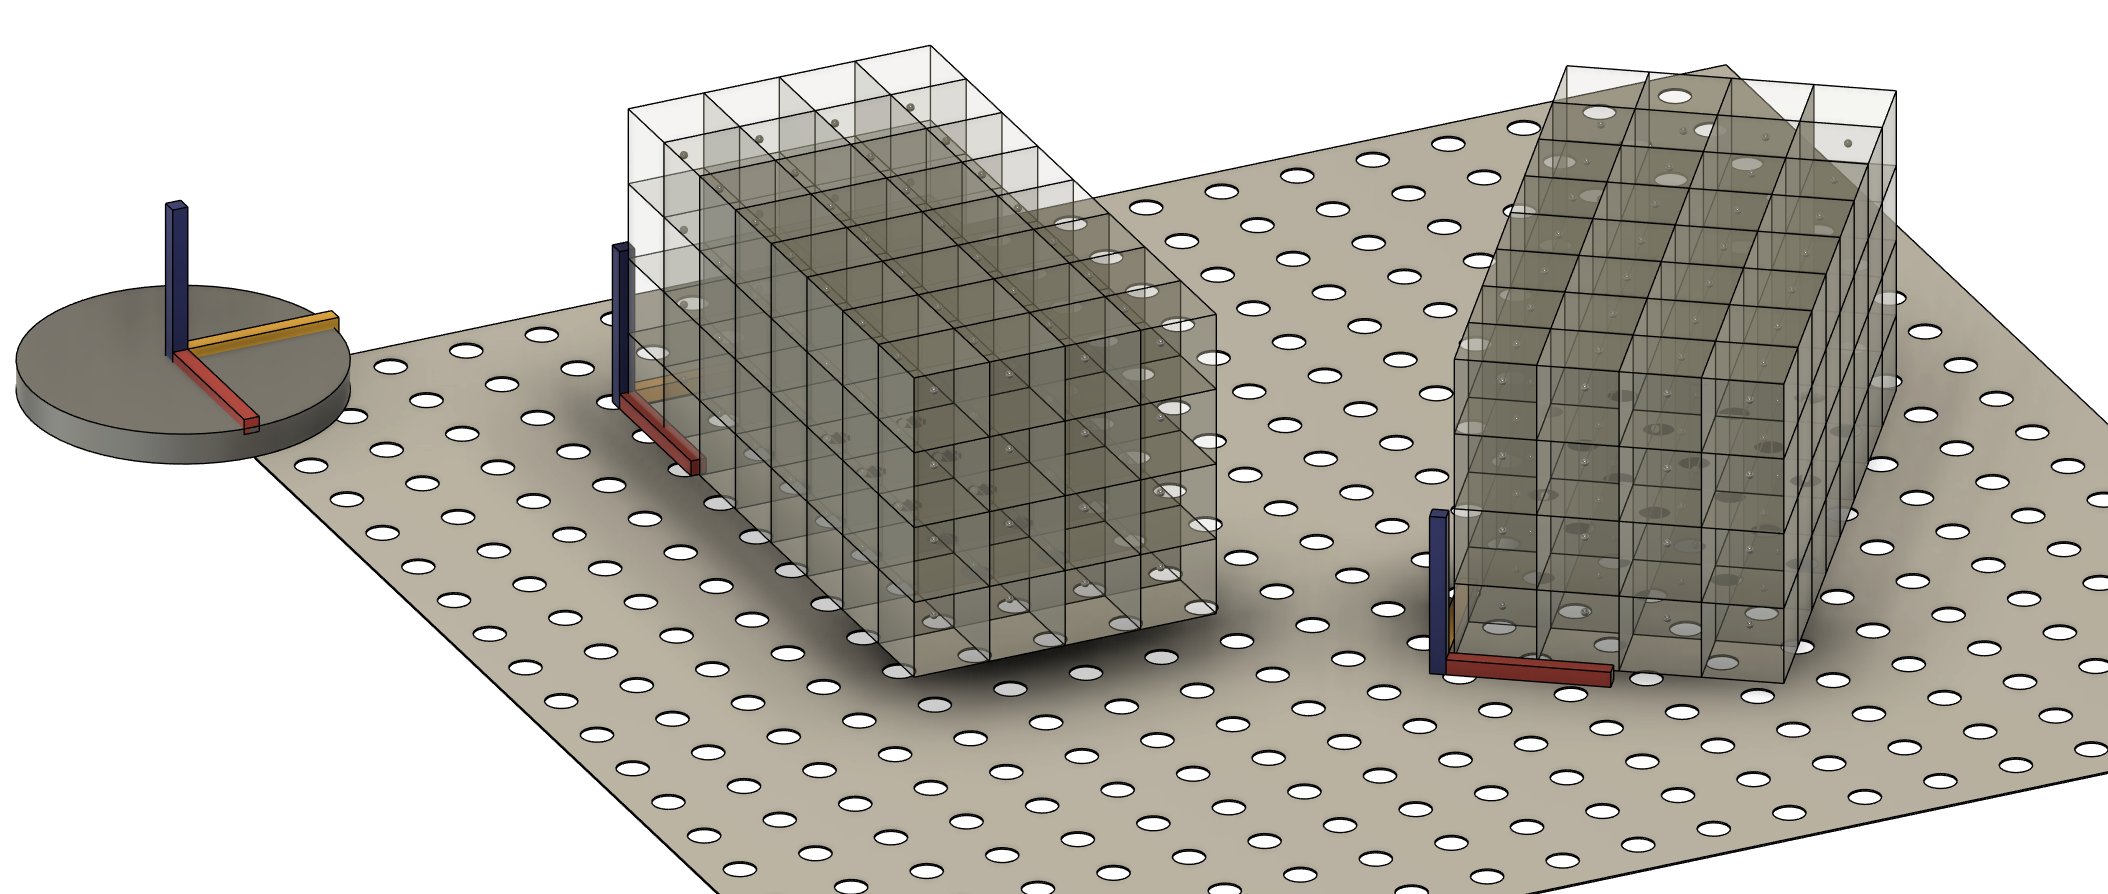
\includegraphics[width=1\textwidth]{grid.PNG}
    \caption{ The figure shows the grid system seen from the robot point if view. The circle on the left is the
robot base(with rotation), with its coordinate frame shown in red, green, and blue.
The hole-patterned plane is the work table, and the two transparent boxes
are predefined grids where the robot can operate. Each grid has its
own coordinate frame in one corner, giving its position relative to
the robot base.}
    \label{fig:mit_billede}
\end{figure}





\subsection{Gridsystem}
Now that the method for moving the robot to a coordinate is defined, the next step is to make it place blocks in a grid. To accomplish this, a grid system is needed to raise the abstraction level from coordinates and kinematics to simple 5x5 squares, defined by a translation and rotation relative to the robot base, which is aligned with the table.


\subsubsection{Grid and blocks}
\subsubsection{compilation}
\subsubsection{Computer Vision approximation}
\subsubsection{main system}

